\documentclass[a4paper,12pt]{report}
\usepackage{ctex}
%\usepackage{xeCJK}
\usepackage{times}
\usepackage{setspace}
\usepackage{fancyhdr}
\usepackage{graphicx}
\usepackage{wrapfig}
\usepackage{array}  
\usepackage{fontspec,xunicode,xltxtra}
\usepackage{titlesec}
\usepackage{titletoc}
\usepackage[titletoc]{appendix}
\usepackage[top=30mm,bottom=30mm,left=20mm,right=20mm]{geometry}
\usepackage{cite}
\usepackage{listings}
\usepackage[framed,numbered,autolinebreaks,useliterate]{mcode} % 插入代码
\usepackage{algorithm, algorithmic} %伪代码
\XeTeXlinebreaklocale "zh"
\XeTeXlinebreakskip = 0pt plus 1pt minus 0.1pt

%---------------------------------------------------------------------
%	页眉页脚设置
%---------------------------------------------------------------------
\fancypagestyle{plain}{
	\pagestyle{fancy}      %改变章节首页页眉
}


%---------------------------------------------------------------------
%	章节标题设置
%---------------------------------------------------------------------
\titleformat{\chapter}{\centering\zihao{-1}\heiti}{\chinese{chapter}}{1em}{}
\titlespacing{\chapter}{0pt}{*0}{*6}

%---------------------------------------------------------------------
%	摘要标题设置
%---------------------------------------------------------------------
\renewcommand{\abstractname}{\zihao{-3} 摘\quad 要}

%---------------------------------------------------------------------
%	参考文献设置
%---------------------------------------------------------------------
\renewcommand{\bibname}{\zihao{2}{\hspace{\fill}参\hspace{0.5em}考\hspace{0.5em}文\hspace{0.5em}献\hspace{\fill}}}

%---------------------------------------------------------------------
%	引用文献设置为上标
%---------------------------------------------------------------------
\makeatletter
\def\@cite#1#2{\textsuperscript{[{#1\if@tempswa , #2\fi}]}}
\makeatother

%---------------------------------------------------------------------
%	目录页设置
%---------------------------------------------------------------------
\titlecontents{chapter}[0em]{\songti\zihao{-4}}{\thecontentslabel\ }{}
{\hspace{.5em}\titlerule*[4pt]{$\cdot$}\contentspage}
\titlecontents{section}[2em]{\vspace{0.1\baselineskip}\songti\zihao{-4}}{\thecontentslabel\ }{}
{\hspace{.5em}\titlerule*[4pt]{$\cdot$}\contentspage}
\titlecontents{subsection}[4em]{\vspace{0.1\baselineskip}\songti\zihao{-4}}{\thecontentslabel\ }{}
{\hspace{.5em}\titlerule*[4pt]{$\cdot$}\contentspage}


\begin{document}
%---------------------------------------------------------------------
%	封面设置
%---------------------------------------------------------------------
\begin{titlepage}
	\begin{center}
		
    
\includegraphics[width=0.9\textwidth]{pic//zju.jpg}\\
    \vspace{10mm}
    \textbf{\zihao{2}\kaishu{计算机科学与技术学院}}\\[0.8cm]
    \textbf{\zihao{2}\kaishu{ 生物智能与算法报告}}\\[3cm]
    
	\vspace{\fill}
	
\setlength{\extrarowheight}{3mm}
{\songti\zihao{3}	
\begin{tabular}{rl}
	
	{\makebox[4\ccwd][s]{姓\qquad 名:}}& ~\kaishu 田若言 \\ 

    {\makebox[4\ccwd][s]{学\qquad 号:}}& ~\kaishu 21721154 \\ 
   
	{\makebox[4\ccwd][s]{老\qquad 师:}} & ~\kaishu 袁昕 \\

\end{tabular}
 }\\[2cm]
\vspace{\fill}
\zihao{4}
2017\textasciitilde 2018春学期\\
使用\LaTeX 撰写于\today
	\end{center}	
\end{titlepage}

%---------------------------------------------------------------------
%  摘要页
%---------------------------------------------------------------------


\begin{abstract}
\begin{spacing}{1.5}
	{\zihao{-4}
	蚁群算法是优化领域中的一种仿生进化算法。该算法采用分布式并行计算机制,具有易与其他方法结合,较强的鲁棒性等特点;但收敛速度慢、易限入局部最优是其突出的缺点。针对蚁群算法,首先介绍其基本原理;然后讨论了蚁群算法的主要缺点和近年来对蚁群算法的若干改进以及在其他领域问题上的应用;最后说明了蚁群算法未来的研究方向和主要研究内容。\\[0.5cm]
	\textbf{关键字}:\quad 蚁群算法 \quad 群聚智能 \quad 觅食行为
	}
\end{spacing}
\end{abstract}

%---------------------------------------------------------------------
%  目录页
%---------------------------------------------------------------------

\tableofcontents % 生成目录




%---------------------------------------------------------------------
%  蚁群算法概述
%---------------------------------------------------------------------
\chapter{蚁群算法概述}
\setcounter{page}{1}


\pagestyle{fancy}
\lhead{\kaishu~生物智能与算法报告~}
\rhead{\kaishu~一.蚁群算法概述~}

\begin{spacing}{1.5}
\songti\zihao{-4}

\section{蚁群算法}
	蚁群优化算法(Ant Colony Optimizer,ACO)是一种模拟蚁群觅食行为的群聚智能算法,由Marco Dorigo等人[1]在1991年提出。Dorigo发现蚁群能通过分泌一种称为信息素的生物激素来交流觅食信息,从而快速的找到目标,据此提出了基于信息正反馈原理的蚁群算法。蚁群算法最初用来解决最短路径问题,在TSP(Traveling Salesman Problem,旅行商问题)上取得了较好的成果。现在也已渐渐应用到其他领域中,在图着色、车辆调度、集成电路设计、通讯网络、数据聚类分析等方面都有所应用。但蚁群算法也存在着诸如收敛速度慢、易陷入局部最优等缺点。



\section{蚁群算法的生物学模型}
	蚂蚁在进行觅食、筑巢等行为过程中,会在所经过的路径上散播一种叫做信息素的物质。而蚂蚁能够感知这种物质的存在及其存在的强度,并以此来指导下一步的运动方向。蚂蚁往往更倾向于向信息素强度较高的方向移动。所以,由大量蚂蚁组成的蚁群便表现出一种信息素正反馈的现象:当某条路径上的蚂蚁越多,该条路径上的信息素就越大,其它蚂蚁选择该条路径的概率就越大。蚂蚁正是通过这种方式,找到一条从蚁巢到食物源之间的最短路径。 
	
\begin{figure}[htbp]
		\centering
		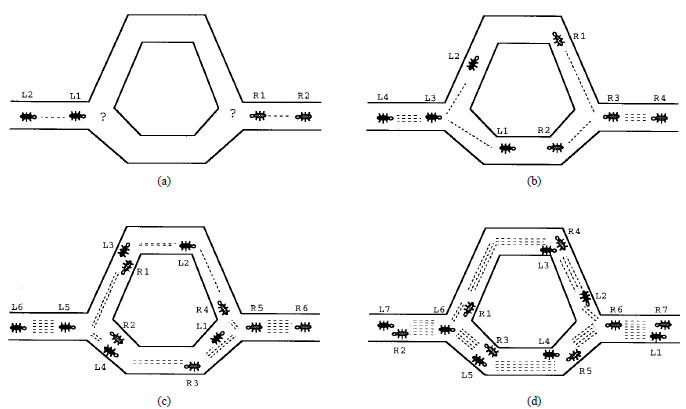
\includegraphics[width=0.6\textwidth]{pic/ant1.png}
		\caption{蚂蚁的觅食行为}
		\label{fig:pt1}
\end{figure}

	Dorigo曾经做过一个双桥实验可以说明这一过程,如图1.1所示。其中(a) (b)中地面上没有信息素的指示,当蚂蚁遇到叉路口时,由于当前路径上没有信息素的指引,所以他们会随机地进行路径选择。在经过一段时间之后,由于下面的路径较上面的路径更短,相同时间内会有更多的蚂蚁通过,下面路径上的信息素积累得会更快,所以越来越多的蚂蚁会选择下面的路径,而这又增强了下面路径上的信息素水平。对于新进入该路径的蚂蚁,它们会以较大概率选择下面的路径,如图 1.1(c)和(d)所示,图中虚线表示路径上信息素的强度。随着时间的推移,下面路径上信息素不断积累,最后几乎所有的蚂蚁都会聚集到该条路径上来。

	基于这样的蚂蚁觅食模型,Dorigo就提出了蚁群算法。

\end{spacing}



%---------------------------------------------------------------------
%  蚁群算法原理
%---------------------------------------------------------------------
\chapter{蚁群算法原理}

\pagestyle{fancy}
\lhead{\kaishu~生物智能与算法报告~}
\rhead{\kaishu~二.蚁群算法原理~}

\begin{spacing}{1.5}
\songti\zihao{-4}

\section{问题定义}
	蚁群算法包含两个基本阶段:适应阶段和协作阶段。在适应阶段,各候选解根据积累的信息不断调整自身结构;在协作阶段,候选解之间通过信息交流,以期产生性能更好的解。
	
	为更清楚地理解蚁群算法的基本原理,一般多借助于经典的对称TSP问题来进行说明。
	
	假设$C=\left\{c_1,c_2,…,c_n \right\}$是图$G$中$n$个城市的集合, $L=\left\{l_{ij}|c_i,c_j\subset C \right\}$是集合$C$中元素(城市)两两连接的集合, $d_{ij}(i,j=1,2,…,n)$是$l_{ij}$的欧几里得距离,$G=(C,L)$是一个无向完全图,TSP问题的目的是从完全图$G$中找出距离最短的哈密顿回路。 

	设$\tau_{ij}(t)$为$t$时刻路径$(i,j)$上的信息素数量,m是所有蚂蚁的数量。$\Gamma =\left\{ \tau_{ij}(t)|c_i,c_j\subset C \right\}$是$t$时刻集合$C$中元素两两连接$l_{ij}$上的残留信息素数量集合,在初始时刻各条路径上信息素数量相等。蚁群算法的寻优是在无向图$g=(C,L,r)$上通过3个准则加以实现,即转移概率准则、局部调整准则和全局调整准则。

	图2.1就是一个TSP问题的完全图。
	\begin{figure}[htbp]
		\centering
		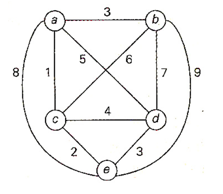
\includegraphics[width=0.4\textwidth]{pic/ant2.png}
		\caption{完全图$G$}
		\label{fig:pt1}
	\end{figure}

\section{概率转移准则}
	蚂蚁$k(k=1,2,…,m)$在运动过程中,根据各条路径信息素数量决定转移方向。算法中人工蚂蚁与实际蚂蚁不同,具有记忆功能。	

	禁忌表$tabu_k(k=1,2,…,m)$用来记录蚂蚁$k$当前所走过的城市。在搜索过程中,蚂蚁根据各个路径上的信息素数量和路径的启发信息来计算转移概率。$p_{ij}^k(t)$表示在$t$时刻蚂蚁$k$由元素$i$转移到元素$j$的转移概率,即:

	%\begin{Large}
	\begin{equation}
		P_{ij}^k(t) = \left\{  
			\begin{array}{lr}  
			   \frac{\tau_{ij}(t) \cdot \eta_{ij}(t)^\beta}{\sum \tau_{is}(t) \cdot \eta_{is}(t)^\beta}\ ,if \ s \subset allowed_k &  \\  
			   0\ , otherwise    
			 \end{array}  
			 \right. 
	\end{equation}
	%\end{Large}
	
	其中:$allowed_k = \left\{C-tabu_k \right\}$表示蚂蚁下一步可以选择的城市,可调参数$\beta (\beta>0)$,决定了$\tau$和$\eta$之间的权重,$\eta_{ij}(t)$为启发函数,即:
	
	\begin{equation}
		\eta_{ij}(t) = 1/d_{ij} 
	\end{equation}

	显然,该启发函数表示了蚂蚁从元素(城市)$i$转移到元素(城市)$j$的期望程度。

	
		

\section{局部调整准则}
	局部调整是每只蚂蚁在建立一个解的过程中进行的。经过$h$个时刻,两个元素状态之间的局部信息素数量要根据下式作调整:
	
	\begin{equation}
		\tau_{ij}(t+h) = (1-\alpha)\cdot\tau_{ij}(t)+\alpha \cdot \tau_0
	\end{equation}

	\begin{equation}
		\tau_0 = 1/(nl_{min})
	\end{equation}
	
	其中:可调参数$0<\alpha<1$,$l_{min}$表示集合C中两个最近元素之间的距离。



\section{全局调整准则}
	只有生成了全局最优解的蚂蚁才有机会进行全局调整,全局调整规则为:
	
	\begin{equation}
		\tau_{ij}(t+n) = (1-\rho) \cdot\tau_{ij}(t)+ \rho \cdot \Delta \tau_{ij}(t)
	\end{equation}

	\begin{equation}
		\Delta \tau_{ij}(t) = \sum_{k=1}^{m} \Delta \tau_{ij}^k(t)
	\end{equation}

	其中:$\rho$为挥发系数,$0< \rho <1$;$\Delta \tau_{ij}(t)$表示本次循环中路径$ij$上的信息素数量的增量;$\Delta \tau_{ij}^k(t)$表示第忌只蚂蚁作本次循环中留在路径$ij$上的信息量。

	文献[1]中曾给出3种不同的蚁群算法模型:Ant-Cycle,Ant-Quantity及Ant-Density,它们的差别在于$\Delta \tau_{ij}(t)$求法的不同:Ant-Cycle利用的是整体信息,在求解TSP问题时性能较好;而Ant-Quantity和Ant-Density利用的是局部信息。因而通常采用Ant-Cycle作为基本模型,即:

	\begin{equation}
		\Delta \tau_{ij}^k(t) = \left\{  
			\begin{array}{lr}  
			   Q/L_k\ ,if \ path(i,j)\ has\ been\ visited\ by\ ant\ k &  \\  
			   0\ , otherwise    
			 \end{array}  
			 \right. 
	\end{equation}

	其中:$Q$是信息素强度,它影响算法的收敛速度;$L_k$表示第$k$只蚂蚁在本次循环中所走路径总长度。



\section{整体算法}
	蚁群优化算法的伪代码如下所示:
	\begin{algorithm}[H]
	\caption{ACO}\label{wolf_alg}
	\algsetup{linenosize=\tiny} \scriptsize
		\begin{algorithmic}
			\STATE{Initialize}
			\STATE{\textbf{Loop /* at this level each loop is called an iteration */}}
				\STATE{$\qquad$Each ant is positioned on a starting node}
				\STATE{\textbf{$\qquad$Loop /* at this level each loop is called a step */}}
					\STATE{$\qquad\qquad$Each ant applies a state transition rule to incrementally build a solution and a local pheromone updating rule}
				\STATE{$\qquad$\textbf{Until} all ants have build a complete solution}
				\STATE{$\qquad$A global pheromone updating rule is applied}
			\STATE{\textbf{Until} End conditon}
		\end{algorithmic}
	\end{algorithm}

	整体算法的思路是将$m$个蚂蚁放在起始点上,每个蚂蚁都会重复的运用概率转移原则去构建一个解,在构建解的过程中,蚂蚁每走过一条边,就会运用局部更新准则去更新边上的信息素。当所有的$m$个蚂蚁都构建了解之后,运用全局更新准则再次更新边上的信息素。

\end{spacing}



%---------------------------------------------------------------------
%  蚁群算法的缺点及改进
%---------------------------------------------------------------------
\chapter{蚁群算法的缺点及改进}
\pagestyle{fancy}
\lhead{\kaishu~生物智能与算法报告~}
\rhead{\kaishu~三.蚁群算法的缺点及改进~}


\begin{spacing}{1.5}
\section{缺点}
	蚁群算法在最短路径问题上能提供有效的解决办法,但也存在着收敛速度慢、易陷入局部最优的缺点。收敛速度慢是因为算法初期信息素匮乏,信息素不能有效的指导搜索过程;易陷入局部最优是因为当算法运行后期信息素累积在局部最优解上,就算发现了更优的路径,这条路径上信息素会比较少,不足以影响整个蚁群的判断。

	针对这些缺点,后续的研究也在蚁群算法上提出了许多改进。

		

\section{改进}
	
\subsection{MMAS}
	MMAS(MIN-MAX Ant System)方法是将信息素浓度被人为的规定在[MIN,MAX]之间,防止信息素过少或者过多,降低局部最优出现的可能性。

\subsection{局部搜索算法2-opt}
	局部搜索算法2-opt(2-Optimization)的基本思想是对当前问题的一个解中任意2个元素进行位置互换,产生另外的解。将新产生的解带入原问题中,取更优的解作为新的最优解。2-opt可以对陷入局部最优的路径进行调整,是组合优化问题中常用的一种手段。图3.1就是2-opt算法的执行过程,通过交换已有解中两个元素的位置,从而发现了新的更优的解。
	\begin{figure}[htbp]
		\centering
		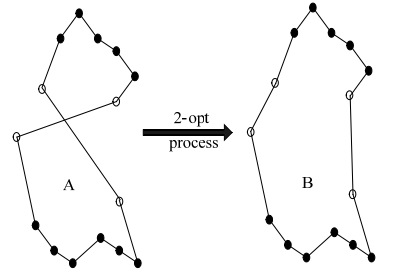
\includegraphics[width=0.4\textwidth]{pic/ant5.jpg}
		\caption{2-opt}
		\label{fig:pt1}
	\end{figure}


\subsection{启发式信息修正}
	启发函数可以在蚂蚁搜索路径的过程中产生一定的影响,比如在第二节提到的蚁群算法中,启发函数是距离的倒数,这就说明蚂蚁在选择下一步要去往的城市时,不仅会考虑地上的信息素,还会考虑当前城市与所选城市之间的距离。但是随着搜索过程的不断深入,较好路径上的信息素的积累越来越多,启启发函数的影响程度也会越来越弱。据此就提出了启发式信息修正[4]的改进方法。
	
	定义\textbf{路径期望值:}所有的$m$只蚂蚁完成一次周游以后,将这次所有的搜索路径按照长度递增的顺序排序,设为$p_1$,$p_2$,$…$,$p_r$,$r(r<m)$是有效路径的数目(可能有多只蚂蚁走同一条路),我们定义蚁群下次周游时的路径期望值为:
	\begin{equation}
	P_{Expect}= \sum_{i=1}^{r} (r+1-i)\times p_i/r
	\end{equation}
这个路径期望值是有效路径的加权平均,权值按照路径的长度来确定。

	算法后期为了避免不必要的搜索,我们提供一个剪枝策略:蚂蚁每次访问一个城市以后,立刻计算已访问路径的长度。如果当前路径长度已经超过路径期望值,则停止对当前路径的后继搜索。对于不满足停止搜索条件的路径(当前路径长度小于路径期望值的那些路径)调整启发函数,调整规则为:
	\begin{equation}
		D_{ij} = \left\{  
			\begin{array}{lr}  
			   P_{Expect}-P_{Visited}-d_{ij},\ if \ (P_{Expect}-P_{Visited}-d_{ij})>0 &  \\  
			   0,\ otherwise    
			 \end{array}  
			 \right. 
	\end{equation}
	\begin{equation}
	\eta_{ij} = \frac{D_{ij}}{\sum D_{is}},\ s\subset allowed_i
	\end{equation}

	由式(4)可知,蚂蚁选择下一个访问城市时,不仅需要考虑当前城市与所选择城市之间的距离,还是考虑本次迭代的路径期望值和当前路径长度。如果访问的下一个城市导致当前路径长度将大于路径期望值,那么这个城市将不会被选择(选择的概率为0)。

\subsection{蚁群算法与其他仿生算法结合}
	将蚁群算法与其他仿生算法进行融合是一个较活跃的应用改进领域。研究最早、最多的是将蚁群算法与遗传算法(Genetic Algorithm ,GA)相结合[3],先用GA初步寻优,找出最优的蚁群算法参数设置,为蚁群算法提供较好的信息素初始分布,再采用蚁群算法进一步寻优以提高算法的收敛速度和全局寻优能力。也有学者将带有人工免疫特性的蚁群算法用于求解连续空间的多模型函数优化问题。

\end{spacing}


%---------------------------------------------------------------------
%  群算法的其他应用
%---------------------------------------------------------------------
\chapter{蚁群算法的其他应用}


\pagestyle{fancy}
\lhead{\kaishu~生物智能与算法报告~}
\rhead{\kaishu~四.蚁群算法的其他应用~}


	蚁群算法在其他许多组合优化问题中也有较好的应用,比如图着色、车辆调度、集成电路设计、通讯网络、数据聚类分析等方面,下面以车辆路径规划[2]和图着色问题[5]为例说明蚁群算法在这两个方面的主要求解思路。

\begin{spacing}{1.5}
	
\section{车辆路径规划问题}
	车辆路径规划问题是由一个车场的车辆向多个客户进行配送服务的问题。在已知车场和客户的位置、客户的需求量以及车辆的数量和最大负载的前提下,设计车辆配送路线满足所有客户的需求,使运输成本最小化,即总代价最小(行车总距离最短或耗费时间最少)。一个车辆路径规划问题的优化路径如图4.1所示:
	\begin{figure}[htbp]
		\centering
		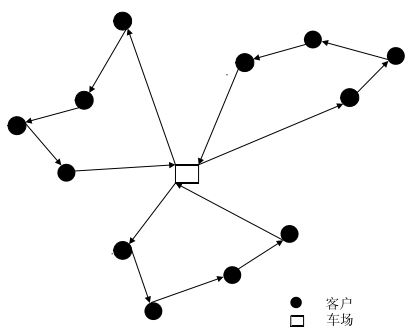
\includegraphics[width=0.5\textwidth]{pic/ant6.jpg}
		\caption{优化路径}
		\label{fig:pt1}
	\end{figure}
	
	利用蚁群算法求解车辆路径规划问题时,一般将蚂蚁看作服务车辆,信息素$\tau_{ij}$表示车辆处于客户$i$时,客户$j$对车辆的吸引程度。在车辆负载满足的条件下,车辆根据路径选择策略选择客户,否则就返回车场,重新选择客户。如果车辆完成所有的客户选择时,算法对每个车辆所构建的路径进行局部搜索,然后对当前路径上的信息素进行更新,从而就完成一次迭代。当算法经过数次迭代后,可以得到一个优化解。

\section{图着色优化问题}
	图着色优化问题的定义是给定无向连通图$G$和$m$种不同的颜色,用这$m$种颜色给$G$中各顶点着色,使得$G$中任意两个相邻顶点的颜色不同,求满足条件的$m$的最小值。

	给定无向图$G(V, E)$,用$m$只蚂蚁对其进行遍历着色,$C={c_1,c_2,c_3,…,c_p}$表示颜色集.每只蚂蚁会维持一张着色表$S(n \times p)$,记录蚂蚁的着色过程,因此也叫着色矩阵,满足:
	\begin{equation}
		S(i,j) = \left\{  
			\begin{array}{lr}  
			  0\ ,v_i\ is\ painted \ with\ color \ c_j &  \\  
			   1\ , v_i\ is\ not\ painted \ with\ color \ c_j    
			 \end{array}  
			 \right. 
	\end{equation}
	且$\sum_{j=1}^{p}S(i,j)=1$。

	所有的蚂蚁共同维持一张信息素表$\tau (n\times p)$,$\tau (i,j)$表示$v_i$着$c_j$色的信息素数量,与着色矩阵$S(n \times p)$相对应。$\Delta_k \tau (i,j)$表示蚂蚁$k$给$v_i$着$c_j$色时释放的信息素数量。

	图着色问题中信息素更新准则为:

	\begin{equation}
	\tau (i,j)= (1-\rho)\cdot \tau(i,j)+\rho \cdot \Delta \tau(i,j)
	\end{equation}

	\begin{equation}
	\Delta \tau(i,j) = \sum_{k=1}^{m}\Delta_k \tau(i,j)
	\end{equation}

	\begin{equation}
	\Delta_k \tau(i,j) = Q/Num_c
	\end{equation}
	其中$Num_c$表示$v_(i-1)$着色后使用的总颜色数。

	蚂蚁在着色遍历时,给vi着cj色的转移准则为:
	\begin{equation}
		P_k(i,j) = \left\{  
			\begin{array}{lr}  
			  \frac{\tau (i,j)^\alpha \cdot \eta ((i,j)^\beta}{\sum \tau (i,j)^\alpha \cdot \eta (i,j)^\beta},if\quad c_j \subset allowed_i^k &  \\  
			   0, otherwise    
			 \end{array}  
			 \right. 
	\end{equation}

	其中$allowed_i^k$表示蚂蚁$k$给$v_i$着色时在已着色集中的可行着色集,它在每次迭每只蚂蚁开始遍历时都为空集。可行着色集为对图着色的约束条件的情况下,从已经用过的颜色集合中取出的符合对$v_i$着色条件的所有颜色的集合。
	
	对$v_i$进行着色时先判断$allowed_i^k$是否为空集,若不为空集则由转移准则给出$v_i$着$c_j$色的概率;若为空集,则$Num_c= Num_c+1$,给$v_i$着$c_Numc$色,并将$c_Numc$放到已经使用过的颜色集合中。


\end{spacing}


%---------------------------------------------------------------------
%  发展与展望
%---------------------------------------------------------------------
\chapter{发展与展望}

\pagestyle{fancy}
\lhead{\kaishu~生物智能与算法报告~}
\rhead{\kaishu~五.发展与展望~}

	蚁群算法是一种原理相对简单的仿生进化算法,在组合优化领域中已展现出它的特点和魅力。但蚁群算法的缺点也非常明显,实际应用也远未挖掘出其真正潜力,还有很多富有挑战性的课题亟待解决。主要体现在以下几个方面:

	1)加强蚁群算法的基础理论研究,包括对解决不同优化问题时收敛性和收敛速度的估计、避免陷入局部最优值、鲁棒性分析以及$\alpha$,$\beta$,$\rho$,$Q$等参数的设计理论。因此,该算法的数学基础理论研究将成为今后研究的一个重要课题。
	
	2)可将蚁群算法与其他类型方法综合使用以开发混合优化方法,进而发展思想更先进、功能更强大、解决更复杂系统的智能行为。目前在解决TSP问题上,蚁群算法已经与遗传算法、免疫算法等有了较好的融合。将蚁群算法与神经网络、模糊控制等相融合,将成为今后蚁群算法领域内新的研究热点。

	3)近年来,蚁群算法虽在许多其他领域的问题上得到了推广应用,但其中大多仅仅是对蚁群算法在该领域应用的一个简单仿真。因此,今后应充分挖掘蚁群算法在实际应用中的潜力,在对现有应用领域进行深化研究的同时,进一步扩大其应用范围。此外,蚁群算法的硬件实现也将成为研究的热点方向之一。

	对上述问题的深入研究必将大大促进蚁群算法理论和应用的发展,蚁群算法也必将在智能计算领域中展现出更加光明的前景。


%---------------------------------------------------------------------
%  参考文献设置
%---------------------------------------------------------------------
\addcontentsline{toc}{chapter}{参考文献}


\begin{thebibliography}{99}
\songti \zihao{-4} 	


\pagestyle{fancy}
\lhead{\kaishu~生物智能与算法报告~}
\rhead{\kaishu~参考文献~}

	\bibitem{Dorigo.{1994}}
	Marco Dorigo. Ant Colony System: A Cooperative Learning Approach to the Traveling Salesman Problem, IEEE TRANSACTIONS ON EVOLUTIONARY COMPUTATION,1997,1(1):53-56.
	
	\bibitem{王沛栋.{2012}}
	王沛栋.改进蚁群算法及在路径规划问题的应用研究[D]山东:中国海洋大学,2012.

	\bibitem{刘波.{2010}}
	刘波.蚁群算法的改进及应用研究[D]河北:燕山大学,2010.

	\bibitem{刘全.{2012}}
	刘全,陈浩,张永刚.一种动态挥发率和启发式修正的蚁群优化算法[J].计算机研究与发展,2012,49(3):620-627.

	\bibitem{朱虎.{2010}}
	朱虎,宋恩民,路志宏.求解图着色问题的最大最小蚁群搜索算法[J].计算机仿真,2010,27(3):190-192.

	
\end{thebibliography}

	

\end{document}